\chapter{مقدمه}
\label{chapter:introduction}

در این فصل به کلیت مسئله‌ی کدگذاری اندیس میپردازیم. با تاریخچه تحقیقاتی و کاربرها و اهمیت آن در صنعت و تعریف دقیق ان آشنا میشویم.
\pagebreak

\section{مقدمه}
کدگزاری اندیس در سال ۱۹۸۸ توسط 
\lr{Birk}
و
\lr{Kol}
در
\cite{25}
هنگام بررسی ارتباطات ماهواره‌ای معرفی شد.  پس از آن مسئله‌ی کدگذاری اندیس کاربردهای متعددی در مسائل مختلف نظری و عملی پیدا کرد. این موضوع باعث شده طی دو دهه گذشته ابزارهای مختلفی از بخش‌های مختلف ریاضی مانند نظریه گراف نظریه، نظریه کدگذاری و نظریه اطلاعات برای توسعه آن استفاده شوند.

	با وجود کاربردهای گوناگون این مسئله، همان طور که در فصل سوم خواهیم دید این مسئله
\transf{ان‌پی-سخت}{NP-Hard}
است و در نتیجه امیدی به حل آن در حالت کلی آن نیست. برای همین سویه‌های مختلفی برای آن توسعه داده شده است که هر کدام مدل یک مسئله‌ی دنیای واقعی هستند.

در این فصل ابتدا با تعریف مقدماتی کدگذاری اندیس(و نه کدگذاری اندیس منعطف)آشنا می‌شویم. کدگذاری اندیس منعطف که موضوع اصلی این پایان‌نامه است یکی از گونه‌های مسئله‌ی کلی تر کدگذاری اندیس است. به دلیل شباهت آن‌ها و برای آشنا شدن با فضای مسئله‌ی اصلی و فهمیدن اینکه چرا گونه‌های مختلف برای این مسئله ایجاد شده است در این فصل به مسئله‌ی کدگذاری اندیس می پردازیم و از فصل بعد به مسئله کدگذاری اندیس منعطف میپردازیم.

 بعد از معرفی مسئله‌ی کدگذاری اندیس در این فصل مرور کوتاهی بر کاربردهای این مسئله میکنیم و با تاریخچه پژوهشی آن آشنا می‌شویم. در بخش پایانی این فصل نیز ساختار این پایان نامه را شرح میدهیم.

\section{تعریف مسئله}
مسئله را با یک مثال توضیح می‌دهیم.
فرض کنید مطابق شکل زیر
\begin{figure}[H]
	\centering
	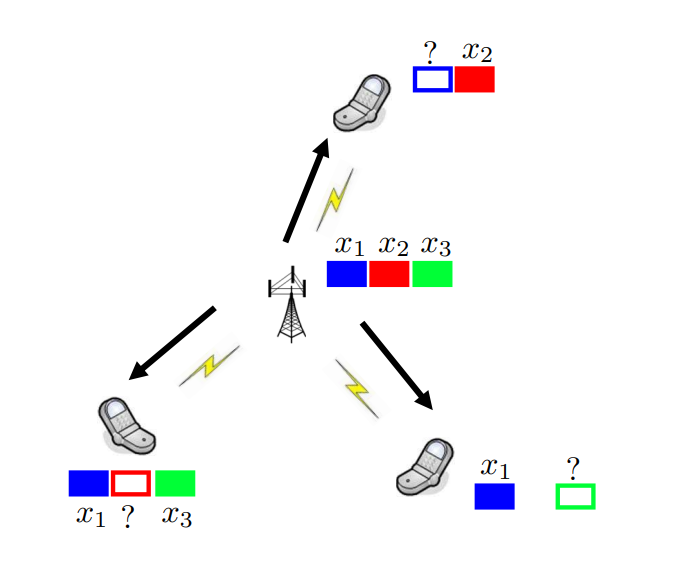
\includegraphics[width=0.7\linewidth]{figs/chapter1/fatemeh1}
	\caption{\cite{Arbabjolfaei2018FundamentalsOI}}
	\label{fig:fatemeh1}
\end{figure}

یک ماهواره‌‌ی رسانه‌ای در حال ارسال اطلاعات برای خبرنگار مختلف است. هر خبرنگار بسته به موقعیت مکانی خود و ارتباط دیگری که دارد از تعدادی از خبرهای روز مطلع است و به دنبال یک خبر جدید است که از آن اطلاعی ندارد تا برای مخاطب محلی خود بازگو کند. ماهواره در هر لحظه میتواند یکی از خبرهای روز را از طریق امواج به سمت کره‌ی زمین ارسال کند که در این صورت تمام خبرنگاران آن خبر را دریافت خواهند کرد. اگر خبرنگاری خبری را دریافت کند که از پیش میداند و یا به هر دلیلی به دنبال آن نیست باید صبر کند تا خبر مورد نظر خود را دریافت کند. مثلا در شکل زیر:

\begin{center}
	\begin{tikzpicture}[->, >=stealth, auto, semithick]
		% Set the positions of the nodes
		\node[circle, draw=blue, fill=blue!20, inner sep=0pt] (C1) at (0,2) {$C_1$};
		
		\node[circle, draw=blue, fill=blue!20, inner sep=0pt] (C2) at (1.5,2) {					$C_2$				};
		\node[circle, draw=blue, fill=blue!20, inner sep=0pt] (C3) at (3,2) {$C_3$				};
		
		\node[circle, draw=green, fill=green!20, inner sep=0pt] (B1) at (0,0) {$B_1$};
		\node[circle, draw=green, fill=green!20, inner sep=0pt] (B2) at (1.5,0) {$B_2$};
		\node[circle, draw=green, fill=green!20, inner sep=0pt] (B3) at (3,0) {$B_3$};
			% Draw the edges
			\draw (C1) -- (B2);
			\draw (C1) -- (B3);
			\draw (C2) -- (B1);
			\draw (C2) -- (B3);
			\draw (C3) -- (B1);
			\draw (C3) -- (B2);
		% Position the parts
		\begin{scope}[on background layer]
			\node[fit=(C1) (C2) (C3), draw=blue, fill=blue!10, rounded corners] {};
			\node[fit=(B1) (B2) (B3), draw=green, fill=green!10, rounded corners] {};
		\end{scope}
	\end{tikzpicture}
	\label{first_example}
\end{center}
 اگر خبرنگاران را با
$c_1, c_2, c_3$
و خبرها را با
$x_1, x_2, x_3$
نشان دهیم خبرنگار اول خبر دوم و سوم را میداند و به دنبال خبر اول است. به طور مشابه برای خبرنگاه دوم و سوم هم برقرار است.

کمترین تعداد دفعات ارسال خبر از طرف ماهواره برای اینکه تمام خبرنگاران به پیام مورد نظر خود دست بیابند چند است؟

برای مدل سازی ریاضی مسئله خبرها را با متغیر های تصادفی مدل میکنیم که از الفبای 
$F$
می‌آیند. همچنین پیام‌های ارسال شده توسط ماهواره نیز اعضای همین مجموعه‌اند.  مثلا برای مثال بالا داریم:

$$
	F = F_2 , X = (0, 0, 1)
$$
راه اول برای حل مثال بالا این است که ماهواره خبر مورد نظر هر خبرنگار را به ترتیب ارسال کند. یعنی اگر پیام‌های ارسالی ماهواره را با
$Y= (y_1, y_2, \ldots)$
نشان دهیم در این صورت ارسال
$Y = (0, 0, 1)$
توسط ماهواره باعث می‌شود تمام خبرنگاران به پیام مورد نظر خود برسند و این یعنی به تعداد خبرنگران ارسال پیام نیاز داریم.

راه دیگر این است که ماهواره مقدار
$Y = (y_1)$
که
$y_1 = x_1 + x_2 + x_3$
را ارسال کند. در این صورت خبرنگار اول با در دست داشتن
$x_2, x_3$
و 
$y_1$
که توسط ماهواره ارسال شده و آن را دریافت کرده است با استفاده از فرمول
$y_1 - x_2 - x_3$
میتواند خبر مورد نظر خود را به دست بیاورد. دو خبرنگار دیگر نیز به طور مشابه با همین تک ارسال میتوانند خبر مورد نظر خود را بیابند و در نتیجه تنها با یک ارسال به جای ۳ ارسال، ماهواره می‌تواند نیاز تمام خبرنگاران را رفع کند.

در واقع در مسئله‌ی کدگذاری اندیس
$m$
متغیر تصادفی و
$n$
کاربر داریم که هر کاربر از قبل مقدار بعضی از متغیر ها را میداند و به دنبال مقدار یک متغیر تصادفی دیگر است که مقدار آن را نمی داند.

برای نمایش مسئله از گراف‌های دوبخشی استفاده می‌کنیم. در یک بخش رئوسی متناظر متغییر های تصادفی و در یک بخش رئوسی متناظر کاربرها. به ازای هر کاربری که یکی از متغییر ها را میداند یک یال بین رئوس متناظر از راس کاربر به راس متغییر میکشیم. مانند شکل
\ref{first_example}
.

مسئله کدگذاری اندیس یافتن کمترین تعداد
\transf{
	ارسال
}{
broadcast, transmission
}
لازم توسط ماهواره است به طوری که تمام 
\transf{
	کاربران
}{
	clients
}
اطلاعات مورد نیاز خود را به دست آورند.
\section{تعریف رسمی کدگذاری اندیس}

\begin{definition}
	یک
	$(t_1, \ldots, t_n, r)$
	-اندیس‌کد از اجزای زیر تشکیل میشود:
	\begin{itemize}
		\item [پیام‌ها]
		$n$
		 متغیر تصادفی که به آن‌ها پیام می‌گوییم. که پیام
		  $i$
		  -ام یک بردار 
		  $t_i$
		  تایی از الفبای
		  $\chi$
		  است. یعنی:
		  $x_i = (x_{i1}, \ldots, x_{it}) \in \chi^{t_i}$
		  \item[
		  کدکننده
		  ]
		   یک تابع کدکننده به شکل:
		   $\phi: \prod\limits_{i = 1}^n \chi^{t_i}  \rightarrow \chi^r$
		  \item[
		  کدگشاها
		  ]
		  $n$
		  تابع کدگشا به شکل
		  $$\forall i \in [n]: \psi_i: \chi^r \times  \prod\limits_{j \in A_i} \chi^{t_j} \rightarrow \chi^{t_i}$$
		  به گونه‌ای که برای
		  $\forall x^n \in \prod\limits_{i = 1}^{n} \chi^{t_i}$
		  داشته باشیم:
		  $$\forall i \in [n]: \psi_i(\phi(x^n), x(A_i)) = x_i$$
	\end{itemize}
\end{definition}
شمای کلی تعریف بالا به این شکل است:
\begin{figure}[H]
	\centering
	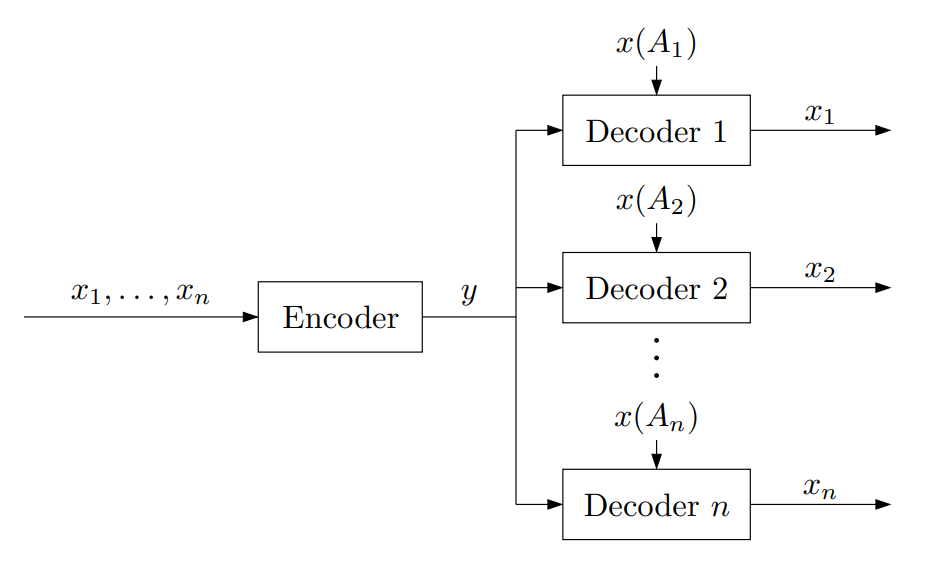
\includegraphics[width=0.7\linewidth]{figs/chapter1/fatemeh2}
	\caption{}
	\label{fig:fatemeh2}
\end{figure}

	به 
	$(t, t, \ldots, t, r)$-اندیس‌کد
	یک
	$(t, r)$-اندیس‌کد
	نیز می‌گوییم.
	
	اگر عمل‌های خطی روی الفبای
	$\chi$
	خوش تعریف باشند برای مثال
	$\chi = \mathbb{F}_q$
	یا یک حلقه(برای مثال حلقه به 
	\cite{Connelly2018}
	مراجعه کنید) و تابع کدگذار و توابع کدگشایی همگی تابع‌هایی خطی باشند به این کد، کد خطی می‌گوییم. اگر 
	$\forall i \in [n] t_i = 1$
	کد اسکالر و در غیر این صورت کد برداری خواهیم داشت. برای مثال در عکس 
	\ref{fig:fatemeh1}
	با یک 
	$(1, 1, 1, 2)$-کد
	مواجه ایم. اگر
	$\chi = \mathbb{F}_2$
	آنگاه خواهیم داشت:
	$$\phi(X) = (Y) \Rightarrow \phi(x_1, x_2, x_3) = (x_1 + x_2, x_3)$$
	و توابع کدگشا نیز
	$$\psi_1 = y_1 + x_2, \psi_2 = y_1 + x_3, \psi_3 = y_2$$
	\begin{definition}[
		نرخ قابل دستیابی
		]
		به چند تایی مرتب
		$(R_1, \ldots, R_n) \ in \mathbb{R}_{\geqslant 0}^n$
		نرخ قابل دستیابی برای مسئله‌ی کدگذاری اندیس گوییم اگر یک 
		$(t_1, \ldots, t_n, r)$-کداندیس
		وجود داشته باشد که
		$$\forall i \in [n]: R_i \leq \frac{t_i}{r}$$
		
		به بستار مجموعه‌ی تمام نرخ‌های قابل دستیابی، ناحیه ظرفیت گویند که با
		$\mathscr{C}$
		نشان می‌دهیم.
	\end{definition}
	
	هدف نهایی  مطالعه کدگذاری یافتن ساختار ناحیه ظرفیت در هر مسئله کدگذاری اندیس و همچنین ساخت یک روش کدگذاری ساده برای دستیابی به آن نرخ‌ها قابل دستیابی است.
	
	به صورت کلی بهینه سای یک پارامتر به بهینه سازی هم‌زمان چند پارامتر ارجحیت دارد برای همین می‌توان از روش دیگری برای نشان دادن ناحیه ظرفیت استفاده کرد.
	\begin{definition}
	برای بردار
	$\mu = (\mu_1, \ldots, \mu_n) \in \mathbb{R}_{\geqslant 0}^n $
	، ناحیه ظرفیت در جهت
	$\mu$
	را به صورت زیر تعریف می‌کنیم:
	$$C(\mu) = max {R: R \mu \in \mathscr{C}}$$
\end{definition}

\begin{remark}
	ناحیه ظرفیت را می‌توان با ناحیه‌های ظرفیت جهت دار بازنویسی کرد:
	$$\mathscr{C} = \bigcup\limits_{\mu} {(R_1, \ldots, R_n): R_i \leq C(\mu) \mu_i, i \in [n]}$$
	ظرفیت متقارن را نیز به صورت زیر تعریف می‌کنیم:
	$$C_{sym} = C(1) $$
\end{remark}

از تعریف ظرفیت متقارن داریم:
$$C_{sym}= \sup\limits_{r} \sup_{(t, r)-code} \dfrac{t}{r} = \lim\limits_{r \rightarrow \infty} \sup_{(t, r)-code} \dfrac{t}{r} $$
که تساوی بین سوپریمم و لیمیت به دلیل زیرجمعی بودن
$$\sup_{(t, r_1 + r_2)-code} t \geqslant \sup_{(t_1, r_1)-code} t_1 + \sup_{(t_2, r_2)-code} t_2$$
و لم
\href{https://en.wikipedia.org/wiki/Subadditivity}{Fekete}
به دست می‌آید.

حال می‌توانیم پارامتری تعریف کنیم به جای بهینه سازی همزمان چند پارامتر فقط یک پارامتر را بهینه کنیم.
\begin{definition}
	نرخ انتشار به صورت زیر تعریف می‌شود:
	$$\beta = \dfrac{1}{C_{sym}}$$
\end{definition}
همچنین داریم:
$$\beta = \inf\limits_{t} \inf\limits_{(t, r) codes} \dfrac{r}{t} = \lim\limits_{t \rightarrow \infty} \inf\limits_{(t, r) codes} \dfrac{r}{t}$$

\begin{remark}
	$$\dfrac{1}{n} \leq C_{sym} \leq 1, 1 \leq \beta \leq n$$
\end{remark}
تا کنون راجع به ناحیه ظرفیت به صورت کلی صحبت کردیم ولی ناحیه ظرفیت برای یک مسئله خاص وابسته به الفبای
$\chi$
انتخاب شده است و بهتر استبه صورت
$\mathscr{C}_\chi$
آن را نمایش بدهیم اما لم زیر نشان می‌دهد که این گونه نیست!
\begin{lemma}
	برای هر دو الفبای متناهی
	$\chi_1, \chi_2$
	داریم:
	$$\mathscr{C}_{\chi_1 }= \mathscr{C}_{\chi_2} $$
\end{lemma}
اثبات این لم در پیوست اول آمده است.
\ref{proof:l1}

هر نمونه از مسئله‌ی کدگذاری اندیس توسط مجموعه‌های اطلاعات جانبی 
$A_1, \ldots, A_n$
به صورت یکتا مشخص می‌شود. در واقع دنباله
$(i, A_i)$
به طور کامل مسئله را مشخص میکند. نمایش های دیگری نیز برای مسئله کدگذاری اندیس وجود دارد. مثلا با استفاده از گراف‌ها می‌توان نمایش‌های گوناگونی ساخت. ما در این جا به ۲ نمایش مختلف را معرفی میکنیم.
\begin{itemize}
	\item 
	$n$
	راس می‌گذاریم. اگر گیرنده‌ی
	$i$-ام
	پیام
	$x_j$
	را به عنوان اطلاعات جانبی بداند از راس
	$v_i$
	به راس
	$v_j$
	یک یال جهت دار میکشیم.
	\begin{figure}[H]
		\centering
		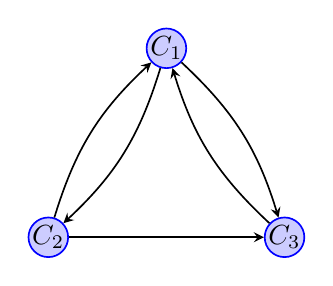
\begin{tikzpicture}[->, >=stealth, auto, semithick]
			% Set the positions of the nodes
			\node[circle, draw=blue, fill=blue!20, inner sep=0pt] (C1) at (0,0) {$C_1$};
			
			\node[circle, draw=blue, fill=blue!20, inner sep=0pt] (C2) at (-1.5,-2.4) {$C_2$};
			\node[circle, draw=blue, fill=blue!20, inner sep=0pt] (C3) at (+1.5,-2.4) {$C_3$};
			% Draw the edges
			\draw (C1) to[bend left=15] (C2);
			\draw (C1) to[bend left=15] (C3);
			\draw (C2)to[bend left=15] (C1);
			\draw (C2) to(C3);
			\draw (C3)to[bend left=15](C1);
		\end{tikzpicture}
			\caption{
		گراف اطلاعت جانبی برای مسئله
		\\
		$A_1 =	\{2, 3\}, A_2 = \{1\}, A_3 = \{1, 2\}$
	}
		\label{fig:fatemeh3}
	\end{figure}
	\item 
	روش بالا برای زمانی است که تعداد پیام‌ها و گیرنده ها برابر باشد. در حالت کلی ممکن است این گونه نباشد. به علاوه روش بالا درک مسئله را سخت‌تر می‌کند. به جای گراف با
	$n$
	رای میتوان از یک گراف دو بخشی با
	$n + m$
	راس استفاده کرد که یک بخش نمایان گر پیام ها و یک بخش نمایانگر گیرنده ها باشد. و به ازای هر گیرنده که یکی از پیام ها را میداند یک یال جهت دار رسم کنیم. این روشی است که در این پایان نامه از آن استفاده میکنیم.
	
	\begin{figure}[H]
		\centering
		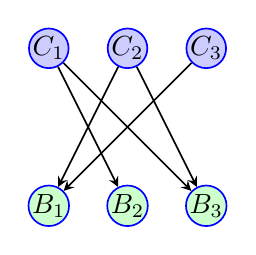
\begin{tikzpicture}[->, >=stealth, auto, semithick]
			% Set the positions of the nodes
			\node[circle, draw=blue, fill=blue!20, inner sep=0pt] (C1) at (0,0) {$C_1$};
			\node[circle, draw=blue, fill=blue!20, inner sep=0pt] (C2) at (1,0) {$C_2$};
			\node[circle, draw=blue, fill=blue!20, inner sep=0pt] (C3) at (+2,0) {$C_3$};
			\node[circle, draw=blue, fill=green!20, inner sep=0pt] (B1) at (0,-2) {$B_1$};
			\node[circle, draw=blue, fill=green!20, inner sep=0pt] (B2) at (1,-2) {$B_2$};
			\node[circle, draw=blue, fill=green!20, inner sep=0pt] (B3) at (2,-2) {$B_3$};
			% Draw the edges
			\draw (C1) to  (B2);
			\draw (C1) to  (B3);
			\draw (C2)to (B1);
			\draw (C2) to(B3);
			\draw (C3)to (B1);
		\end{tikzpicture}
		\caption{
			گراف اطلاعت جانبی برای شکل
			\ref{fig:fatemeh3}
		}
		\label{fig:fatemeh4}
	\end{figure}
\end{itemize}

	تعداد نمونه‌های مسئله‌ی کدگذاری اندیس با
	$n$
	پیام و کلاینت برابر
	$2^{n(n - 1)}$
	است. که برای
	$n$
	های کوچک نیز بسیار سریع رشد می‌کند. حتی حذف گراف‌های یکریخت نیز تاثیری ندارد(برای تعداد گراف‌های یکریخت میتوان به سایت زیر رفت
	\cite{web:unlabeled}
	)
	
	کدگذاری اندیس را می‌توان به صورت حالت خاصی از مسئله‌ی 
	
	\transf{
	کدگذاری شبکه تک‌پخشی چندگانه
	}{
	multiple-unicast network coding
	}[رجوع شود به
	\cite{paper:Networkinformationflow}
	و
	\cite{yeung2008information}
	]
	در نظر گرفت. برای نمونه، شکل
	\ref{fig:fatemeh4}
	 و را می‌توان به شکل زیر در نظر گرفت.
		\begin{figure}[H]
		\centering
		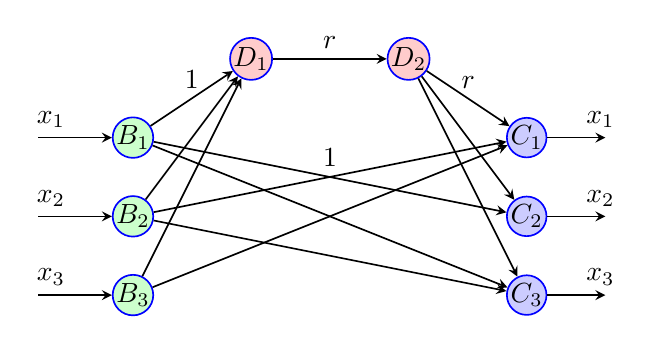
\begin{tikzpicture}[->, >=stealth, auto, semithick]
			% Set the positions of the nodes
			\node[circle, draw=blue, fill=red!20, inner sep=0pt] (D1) at (1.5,1) {$D_1$};
			\node[circle, draw=blue, fill=red!20, inner sep=0pt] (D2) at (3.5,1) {$D_2$};
			
			\node[circle, draw=blue, fill=blue!20, inner sep=0pt] (C1) at (5,0) {$C_1$};
			\node[circle, draw=blue, fill=blue!20, inner sep=0pt] (C2) at (5,-1) {$C_2$};
			\node[circle, draw=blue, fill=blue!20, inner sep=0pt] (C3) at (5,-2) {$C_3$};
			\node[circle, draw=blue, fill=green!20, inner sep=0pt] (B1) at (0,0) {$B_1$};
			\node[circle, draw=blue, fill=green!20, inner sep=0pt] (B2) at (0,-1) {$B_2$};
			\node[circle, draw=blue, fill=green!20, inner sep=0pt] (B3) at (0,-2) {$B_3$};
			% Draw the edges
			\draw (B1) to node[midway,above ] {$1$} (C2);
			\draw (B1) to(C3);
			\draw (B2)to (C1);
			\draw (B2) to(C3);
			\draw (B3)to (C1);
			\draw (D1)to node[midway,above ] {$r$} (D2);
			\draw (B1)to node[midway,above ] {$1$}(D1);\draw (B2)to (D1);\draw (B3)to (D1);
			\draw (D2)to node[midway,above ] {$r$}(C1);\draw (D2)to (C2);\draw (D2)to (C3);
			\draw (-1.2, 0)to node[midway,above left] {$x_1$} (B1) ;\draw (-1.2, -1)tonode[midway,above left] {$x_2$} (B2);\draw (-1.2, -2)tonode[midway,above left] {$x_3$} (B3);
			\draw (C1)to node[midway,above right] {$x_1$}(6,0) ;\draw (C2)to node[midway,above right] {$x_2$}(6, -1);\draw(C3) to node[midway,above right] {$x_3$}(6, -2);
		\end{tikzpicture}
		\caption{
			گراف اطلاعت جانبی برای شکل
			\ref{fig:fatemeh3}
		}
		\label{fig:fatemeh5}
	\end{figure}
	ظرفیت یال‌های میانی و یال‌های ورودی به
	$D_1$
	برابر یک و ظرفیت یال
	$()D_1, D_2)$
	و یال‌های خروجی از
	$D_2$
	برابر
	$r$
	است که همان ظرفیت ارسال ماهواره است. برای توصیف دقیق مسئله‌ی کدگذاری شبکه و اثبات برابر آن با مسئله‌ی کدگذاری اندیس به
	\cite{effros2012equivalence}
	رجوع کنید.
	
	
\section{
	کاربردها، اهمیت و تاریخچه پژوهشی
	}
\subsection{
	مروری بر کاربردها
}

\subsection{
تاریخچه پژوهشی
}
مسئله کدگذاری اندیس توسط بیرک و کول 
\cite{25, 26}
 در زمینه ارتباطات ماهواره‌ای معرفی شد. فرمول‌بندی‌های مرتبط نیز پیشتر در کارهای سلبیلر و استت
  \cite{paper:1455117:Celebiler}،
   واینر، ولف، و ویلمز 
\cite{152}
، و یئونگ 
\cite{158}
 مورد مطالعه قرار گرفته است. اصطلاح "کدگذاری اندیس" توسط بار-یوسف، بیرک، جیرم، و کول 
\cite{4031356}
 به کار برده شده است که مسئله کدگذاری اندیس را با مسئله کدگذاری منبع بدون خطا با اطلاعات جانبی که توسط ویتسنهاوزن
\cite{1055607}
 مطالعه شده است، مقایسه کرده‌اند و این نکته را مشخص کردند که در مسئله کدگذاری اندیس، هدف گیرنده پیدا کردن بخشی از منبع است. در واقع گیرنده به دنبال یک اندیس است. پس، همانند کانال‌های ترکیبی
 \cite{27, 53, 154}
، فرستنده می‌تواند به صورت پیش‌دستانه ارسال خود را کدگذاری کرده و به گیرنده در تمامی پیکربندی‌های ممکن پخش کند
\cite{48}
. علاوه بر ارتباطات ماهواره‌ای، کدگذاری اندیس در زمینه‌های متنوعی مانند توزیع چندرسانه‌ای 
\cite{114}
، مدیریت تداخل 
\cite{81}
، و  کش‌های کدگذاری شده 
\cite{103, 82}
 کاربرد دارد. این مسئله همچنین به بسیاری از مسائل مهم دیگر مانند کدگذاری شبکه 
\cite{122, 61, 59}
، ذخیره‌سازی توزیع‌شده قابل بازیابی محلی 
\cite{108, 128, 13}
، بازی‌های حدس‌زنی در گراف‌های جهت‌دار 
\cite{122, 162, 13}
، نظریه ماتروید 
\cite{61}
، و ظرفیت بدون خطای کانال‌ها 
\cite{131}
 نیز نزدیک است.
به خاطر این اهمیت، مسئله کدگذاری اندیس به طور گسترده‌ای طی دو دهه گذشته مورد مطالعه قرار گرفته است. ابزارهای متنوعی از جمله نظریه گراف، نظریه کدگذاری، و نظریه اطلاعات برای ارائه طرح‌های کدگذاری غیر بدیهی
\cite{25, 101, 22, 43, 114, 29, 8, 104, 81, 130, 7, 9, 149, 116, 80, 141, 146, 162}
و همچنین کران‌‌های بالا و پایین 
\cite{160, 22, 55, 28, 17, 141}
 بکار رفته‌اند.
 
 یکی از مسیرهای پژوهشی تعریف گونه‌های جدید برای مسئله است. برای مثال اگر کلاینت‌ها به جای اینکه به دنبال دریافت یکی از پیام‌ها باشند  به دنبال یک پیام جدیدی که جزو اطلاعات جانبی آن ها نیست باشند به مسئله‌ی کدگذاری اندیس منعطف می‌رسیم که موضوع اصلی این پایان نامه است. برای  دیدن گونه‌های مختلف می‌توان برای مثال به
 \cite{pliablefirstpaper, verypliable, byrne2023preferential}
 رجوع کرد.
 
\section{اهداف و دست‌آورد‌های پژوهشی}
از نظر پژوهش ریاضی در زمینه‌ی کدگذاری اندیس بخش عمده کارها به یافتن کران بالایی برای تعداد پیام مورد نیاز روی گراف‌های مختلف صورت گرفته است. به طور خاص در مسئله‌ی کدگذاری اندیس منعطف به این مسئله تشدید نیز می‌شود و تقریبا کار پژوهشی‌ مهمی روی کران پایین انجام نشده است. هدف اولیه شروع این پژوهش تکمیل این بخش از پژوهش‌ها با یافتن کران پایین برای مسئله‌ی کدگذاری اندیس بود.
%shit

\section{ساختار پایان‌نامه}

این پایان‌نامه در هفت فصل به شرح زیر ارائه می‌شود.
فصل دوم به بیان پیش‌نیازهای علمی مورد نیاز شامل مطالبی پیرامون نظریه گراف، نظریه اطلاعات، جبر خطی و روش‌های احتمالاتی  می‌پردازد.

فصل سوم به مطالعه و بررسی کارهای پیشین با موضوع این پایان‌نامه می‌پردازد. در این فصل به کارهای بنیادی 
\lr{Fragouli}
در زمینه‌ی کدگذاری اندیس منعطف می‌پردازیم و یک الگوریتم چندجمله‌ای قطعی برای مسئله را بررسی میکنیم.

در فصل چهارم، به گونه‌های مختلف مسئله می‌پردازیم و با مقدمات و کاربردهای هر کدام آشنا می‌شویم.

در فصل پنجم، نتایج جدیدی که در این پایان‌نامه به‌دست آمده است، ارائه می‌شود.

فصل ششم ارتباطات مسئله کدگذاری اندیس با مسائل نظری دیگر می‌پردازیم.

در فصل هفتم به جمع‌بندی کارهای انجام شده در این پژوهش و ارائه‌ی پیشنهادهایی برای انجام کارهای آتی خواهیم پرداخت.